\documentclass[10pt,journal,compsoc]{IEEEtran}
% For T-BIOM submission

% Packages
\usepackage{amsmath,amssymb,amsfonts}
\usepackage{algorithm}
\usepackage{algorithmic}
\usepackage{graphicx}
\graphicspath{{../figures/}} % Tell LaTeX where to find figures
\usepackage{textcomp}
\usepackage{xcolor}
\usepackage{cite}
\usepackage{url}
\usepackage{hyperref}
\usepackage{booktabs} % For professional tables
\usepackage{multirow} % For tables with merged cells

% Correct hyphenation
\hyphenation{op-tical net-works semi-conduc-tor com-plex-i-ty en-roll-ment bio-met-ric lon-gi-tu-di-nal as-sump-tions}

\begin{document}

\title{Beta Regression Framework for Modeling Bounded Biometric Performance in Child Face Recognition}

\author{\IEEEauthorblockN{Aaron W. Storey\,\IEEEmembership{Member,~IEEE}}\\
\IEEEauthorblockA{Department of Computer Science\\
Clarkson University\\
storeyaw@clarkson.edu\\
ORCID: 0009-0009-5560-0015}}

\markboth{IEEE Transactions on Biometrics, Behavior, and Identity Science}%
{Storey: Beta Regression for Bounded Biometric Performance}

\maketitle

\begin{abstract}
Child face recognition systems degrade over time, yet standard statistical models can produce nonsensical predictions when modeling this degradation. This paper examines beta regression as an alternative approach for bounded biometric performance metrics. Building on empirical work by Deb et al.~\cite{deb2018} and Bahmani et al.~\cite{bahmani2023}, this analysis identifies a methodological gap: while these studies appropriately use standardized scores, practitioners often need to model raw recognition rates for operational decisions. The simulations show that linear mixed models applied directly to bounded data can predict impossible values---in one case exceeding 100\% true accept rate. Beta regression eliminates these violations while maintaining comparable fit. This pedagogical example illustrates why matching statistical tools to data constraints matters. The approach captures age-dependent patterns naturally: young children (ages 3-5) show rapid performance decline, middle childhood (5.5-7 years) exhibits surprising stability near 80\%, and older children experience delayed degradation after puberty onset. Perhaps most importantly for operational systems, beta regression correctly models the variance structure of bounded data, with uncertainty peaking at 50\% performance. This has practical implications---the analysis suggests the stable middle-age group could use extended re-enrollment intervals, potentially improving resource allocation for missing child searches. Implementation code and guidelines are provided for when this approach offers advantages over traditional methods. Available at: \url{https://github.com/astoreyai/memory-augmented-transformers}.
\end{abstract}

\begin{IEEEkeywords}
Biometric evaluation, bounded outcomes, beta regression, child face recognition, longitudinal analysis, variance modeling, statistical methods
\end{IEEEkeywords}

\IEEEpeerreviewmaketitle

\section{Introduction}
\label{sec:introduction}
\IEEEPARstart{C}{hild} face recognition serves a critical social mission---reuniting missing children with their families. Recent advances in child face recognition include synthetic data generation~\cite{falkenberg2024} and deep feature aging~\cite{deb2021missing} for missing children identification. Yet the statistical models chosen for analyzing performance degradation can lead to errors. Published studies like Deb et al.~\cite{deb2018} wisely use standardized scores that avoid mathematical contradictions. However, when practitioners need to model raw recognition rates for operational decisions, inappropriate application of standard tools can lead to errors. Simulations showed that linear mixed models, when applied directly to bounded performance data, sometimes predict recognition rates above 100\%---a mathematical impossibility that undermines system credibility. This isn't just a theoretical concern; it reflects a fundamental mismatch between the tools and the data.

It is important to note that these issues arise from model misapplication---using tools designed for unbounded data on inherently bounded outcomes---not from flaws in linear models themselves.

Longitudinal studies have identified complex age-dependent degradation patterns that pose challenges for statistical modeling and operational system design. While biometric researchers have developed established evaluation methods---including d-prime analysis, ROC curves, and score normalization techniques---directly modeling raw recognition rates remains valuable for interpretability and policy decisions.

Deb et al.~\cite{deb2018} analyzed 3,682 face images from 919 children aged 2--18 years in their Children Longitudinal Face dataset, tracking subjects irregularly over periods of 2--7 years. Testing multiple algorithms showed consistent degradation patterns: Commercial-Off-The-Shelf~A accuracy dropped from roughly 82\% at one year to 49\% after three years, while FaceNet declined from about 84\% to 60\% over the same period. Their fusion approach performed better initially (90\%) but still fell to 73\% by year three. The team's linear models estimated annual degradation around 0.22 standard deviations across all approaches, using bootstrap methods to handle normality violations. Yet these models carry an inherent assumption---constant variance and symmetric errors---that becomes problematic when dealing with bounded recognition rates, especially during long-term extrapolation.

Bahmani et al.~\cite{bahmani2023} took a different approach, collecting 3,831 images from 330 subjects with rigorous sampling every six months for eight years. Using the MagFace algorithm, they found near-perfect accuracy (over 98\%) at two years that degraded to around 71\% by year eight. The age-specific patterns provided critical insights: young children between 3 and 5 years old showed the steepest decline, dropping from the high 90s to the low 60s. Unexpectedly, children aged 5.5 to 7 years maintained remarkably stable performance around 80\% throughout the study period. Teenagers showed intermediate patterns. Despite these compelling patterns warranting further investigation, the author limited their analysis to descriptive statistics.

These studies highlight a methodological challenge: while effect sizes and transformations can handle bounded outcomes, directly modeling percentage-based performance offers advantages for operational decisions. It is important to note that biometric systems output similarity scores that are thresholded to produce binary decisions. The True Accept Rate (TAR) at a fixed False Accept Rate (FAR) represents the proportion of genuine comparisons exceeding this threshold. While actual systems involve complex score distributions, modeling aggregate TAR values provides interpretable metrics for stakeholders and enables longitudinal performance tracking.\footnote{While TAR represents aggregated performance, it emerges from underlying genuine and impostor score distributions. Beta regression models the aggregate metric directly, trading distributional detail for interpretability.} Beta regression provides a principled approach that respects probability bounds while naturally capturing the mean-variance relationships observed in such bounded biometric data~\cite{ferrari2004}. This paper examines when and how beta regression complements existing biometric evaluation practices, with particular focus on variance modeling and long-term prediction accuracy.

This work bridges a gap between statistical methodology and biometric practice. The analysis identifies when beta regression offers genuine advantages over standard approaches, particularly for long-term predictions and operational planning. Through simulation studies, this paper shows how this method better captures the variance patterns inherent in bounded data---something that becomes critical when making decisions about re-enrollment schedules or resource allocation. Most importantly, practical guidance is provided on when to use this approach versus sticking with established methods, helping researchers match their statistical tools to their specific evaluation needs.

\section{Related Work}
\label{sec:related_work}

Child face recognition presents unique challenges compared to adult systems. Farkas~\cite{farkas1994} documented systematic craniofacial changes during development, establishing the biological foundation for performance degradation. Best-Rowden and Jain~\cite{bestrowden2018} showed adult face recognition remains stable for over a decade, contrasting sharply with child patterns. Huang et al.~\cite{huang2023} developed the MTLFace framework for age-invariant recognition, establishing benchmarks specifically for missing children applications, while Yoon and Jain~\cite{yoon2015} conducted a comprehensive longitudinal study of fingerprint recognition, demonstrating multilevel statistical models for template aging analysis that extend to other biometric modalities.

Statistical modeling of bounded outcomes has evolved significantly. Ferrari and Cribari-Neto~\cite{ferrari2004} introduced beta regression for modeling rates and proportions. Smithson and Verkuilen~\cite{smithson2006} demonstrated beta regression's superiority over transformed linear models for psychological data with heteroscedastic variance. Cribari-Neto and Zeileis~\cite{cribari2010} developed practical implementations in R. Mixed-effects extensions appeared in Brooks et al.~\cite{brooks2017} through the glmmTMB package, while B\"urkner~\cite{burkner2017} enabled Bayesian approaches via brms. Figueroa-Zúñiga et al.~\cite{figueroa2013} extended this framework to Bayesian mixed effects models, enabling robust uncertainty quantification. Hunger et al.~\cite{hunger2012} demonstrated mixed effects beta regression for analyzing bounded longitudinal health scores, providing the methodological foundation for biometric performance tracking. Laird and Ware~\cite{laird1982} established the foundational framework for random-effects models in longitudinal data, enabling proper handling of within-subject correlation structures essential for biometric performance tracking.

Despite these advances, biometric performance modeling remains dominated by linear approaches. This paper bridges the gap between statistical methodology and biometric applications.

\section{Current Biometric Evaluation Practices}
\label{sec:current_practices}

The biometric community has developed several effective approaches for handling performance metrics that naturally fall between 0 and 1. Signal detection theory provides perhaps the most elegant solution through the sensitivity index d-prime ($d'$), which quantifies discriminability independent of decision thresholds. Wu et al.~\cite{wu2011} established rigorous statistical frameworks for operational ROC analysis, addressing uncertainties and significance testing in biometric systems building on the ISO/IEC 19795 standards~\cite{garris2005} for biometric performance testing. By modeling match and non-match scores as normal distributions, this approach sidesteps boundary issues entirely while providing a scale-free performance measure. Receiver Operating Characteristic (ROC) analysis takes a different tack, characterizing the inherent trade-off between False Accept Rate and False Reject Rate across all possible thresholds. Best-Rowden et al.~\cite{bestrowden2013} demonstrated the mathematical relationship between ROC and CMC curves through the biometric menagerie framework, while Adler and Schuckers~\cite{adler2005} developed methods for composite DET curve calculation. The resulting curves, and their associated Area Under the Curve metrics, remain properly bounded while offering threshold-independent evaluation. Score normalization techniques---whether Z-norm, T-norm, or adaptive cohort methods---transform raw similarity scores to account for subject-specific and time-varying distributions. These transformations implicitly respect boundary constraints while improving system calibration. The ISO/IEC 19795-2 standard, comprehensively reviewed by Richiardi and Kryszczuk~\cite{richiardi2011}, establishes evaluation protocols for technology and scenario testing. Recent advances by Schlett et al.~\cite{schlett2024} extend these standards through EDC plots and partial AUC analysis for biometric quality assessment.

When researchers do need to model bounded rates directly, the standard approach involves transformation. Logit and probit transforms map recognition rates to unbounded scales where linear models apply naturally. Back-transformation then returns predictions to the original bounded space. Each method has its place in the biometric evaluation toolkit.

Despite their theoretical elegance, these methods face practical limitations. The interpretability gap remains significant---d-prime values and log-odds ratios, while statistically rigorous, often prove challenging for operational stakeholders who require intuitive percentage-based metrics for resource allocation decisions. Transformations create their own complications. While logit and probit transforms mathematically map bounded data to unbounded scales, they don't preserve the natural variance structure of recognition rates. The variance of a proportion peaks at 50\% and shrinks near the boundaries---a pattern that gets distorted through transformation and back-transformation. This matters when constructing confidence intervals or making probabilistic statements about future performance.

Even with transformations, extreme extrapolation can produce nonsensical results. A model might behave perfectly within the range of observed data, but project it forward ten years and back-transformed predictions can still exceed 100\% or dip below 0\%. Finally, incorporating hierarchical structures with subject-specific random effects becomes mathematically complex in many of these methods, limiting their utility for longitudinal studies where individual variation matters.

Direct modeling of recognition rates becomes essential in several operational contexts. Policy makers need interpretable metrics when allocating resources or setting re-enrollment schedules---telling them a system maintains "82\% accuracy" carries more weight than abstract statistical measures. Age-specific threshold optimization also benefits from direct modeling, as operators can immediately see how performance varies across age groups and adjust system parameters accordingly. Longitudinal studies with substantial individual variation particularly benefit from this approach. When tracking the same children over years, methods are needed that naturally handle both the bounded nature of recognition rates and the hierarchical structure of repeated measurements. Multi-modal biometric systems present another compelling use case, as different modalities (face, fingerprint, iris) often operate on different measurement scales that require careful integration while respecting each modality's natural bounds.

Beta regression addresses these specific use cases while complementing, rather than replacing, established biometric evaluation methods. Beta regression outputs integrate with ISO/IEC 19795-2 evaluation protocols by providing confidence intervals for operational points on the ROC curve.

Having established the current best practices and their appropriate use cases, this section examines specific statistical patterns in longitudinal child face recognition data that indicate opportunities for methodological improvement.

\section{Statistical Challenges in Longitudinal Biometric Data}
\label{sec:challenges}

\subsection{Empirical Evidence from Longitudinal Studies}

Two major longitudinal studies have shaped our understanding of child face recognition degradation, each revealing distinct statistical patterns that challenge traditional modeling approaches. Deb et al.~\cite{deb2018} built a two-level hierarchical model where Level~1 modeled within-subject changes over time and Level~2 captured between-subject variability, assuming linear degradation over time. Their statistical framework appropriately uses standardized scores, reporting annual degradation of 0.2444 standard deviations---an effect size measure (similar to Cohen's d) that avoids boundary issues in their analysis. Their use of standardized outcomes and bootstrap resampling represents sound statistical practice for their research goals. However, when practitioners need to translate such findings to operational TAR values (approximately 6-10 percentage point annual declines), the choice of modeling approach becomes critical. The concern here is not with their methodology, but with how such results might be applied in operational settings where bounded percentage metrics are required for stakeholder communication. Adult face recognition exhibits markedly different patterns---previous work found that 99\% of adults maintained recognition above threshold for 10.5 years~\cite{bestrowden2018}, whereas children exhibited degradation rates three times higher. One model cannot fit both patterns when constrained to bounded outcomes without producing invalid predictions.

Bahmani et al.~\cite{bahmani2023} sampled every 6 months, showing hidden complexity. Multiple age-dependent patterns emerged, each telling a different story about facial development (Figure~\ref{fig:age-patterns}).

The youngest group, ages 3-5, exhibited rapid performance degradation. Starting from near-perfect recognition, their performance declined by 15 percentage points within the first two years---a substantial operational challenge. Following this initial rapid decline, the degradation rate decreased but continued steadily, eventually stabilizing in the low 60s. This pattern suggests exponential rather than linear decay, with rapid initial change followed by gradual stabilization.

The 5.5 to 7-year-old cohort showed unexpected stability. This group maintained remarkably consistent performance, hovering around 80\% accuracy throughout the entire eight-year study. Rather than the anticipated decline, the data showed a plateau---suggesting facial development may experience a period of relative stability during these years.

The older cohort presented a distinct pattern. Their near-perfect initial performance remained stable for approximately four years before experiencing sharp degradation between years four and eight, coinciding with pubertal onset. This delayed degradation pattern---stable performance followed by rapid decline---represents a non-linear trajectory that standard linear models, when applied directly to bounded outcomes, cannot capture adequately.

The authors stated: ``accuracy performance does not exhibit consistent trends with increasing age within enrollment age groups''~\cite{bahmani2023}. This finding directly contradicts the assumptions of linear models.

\begin{figure}[htbp]
\centering
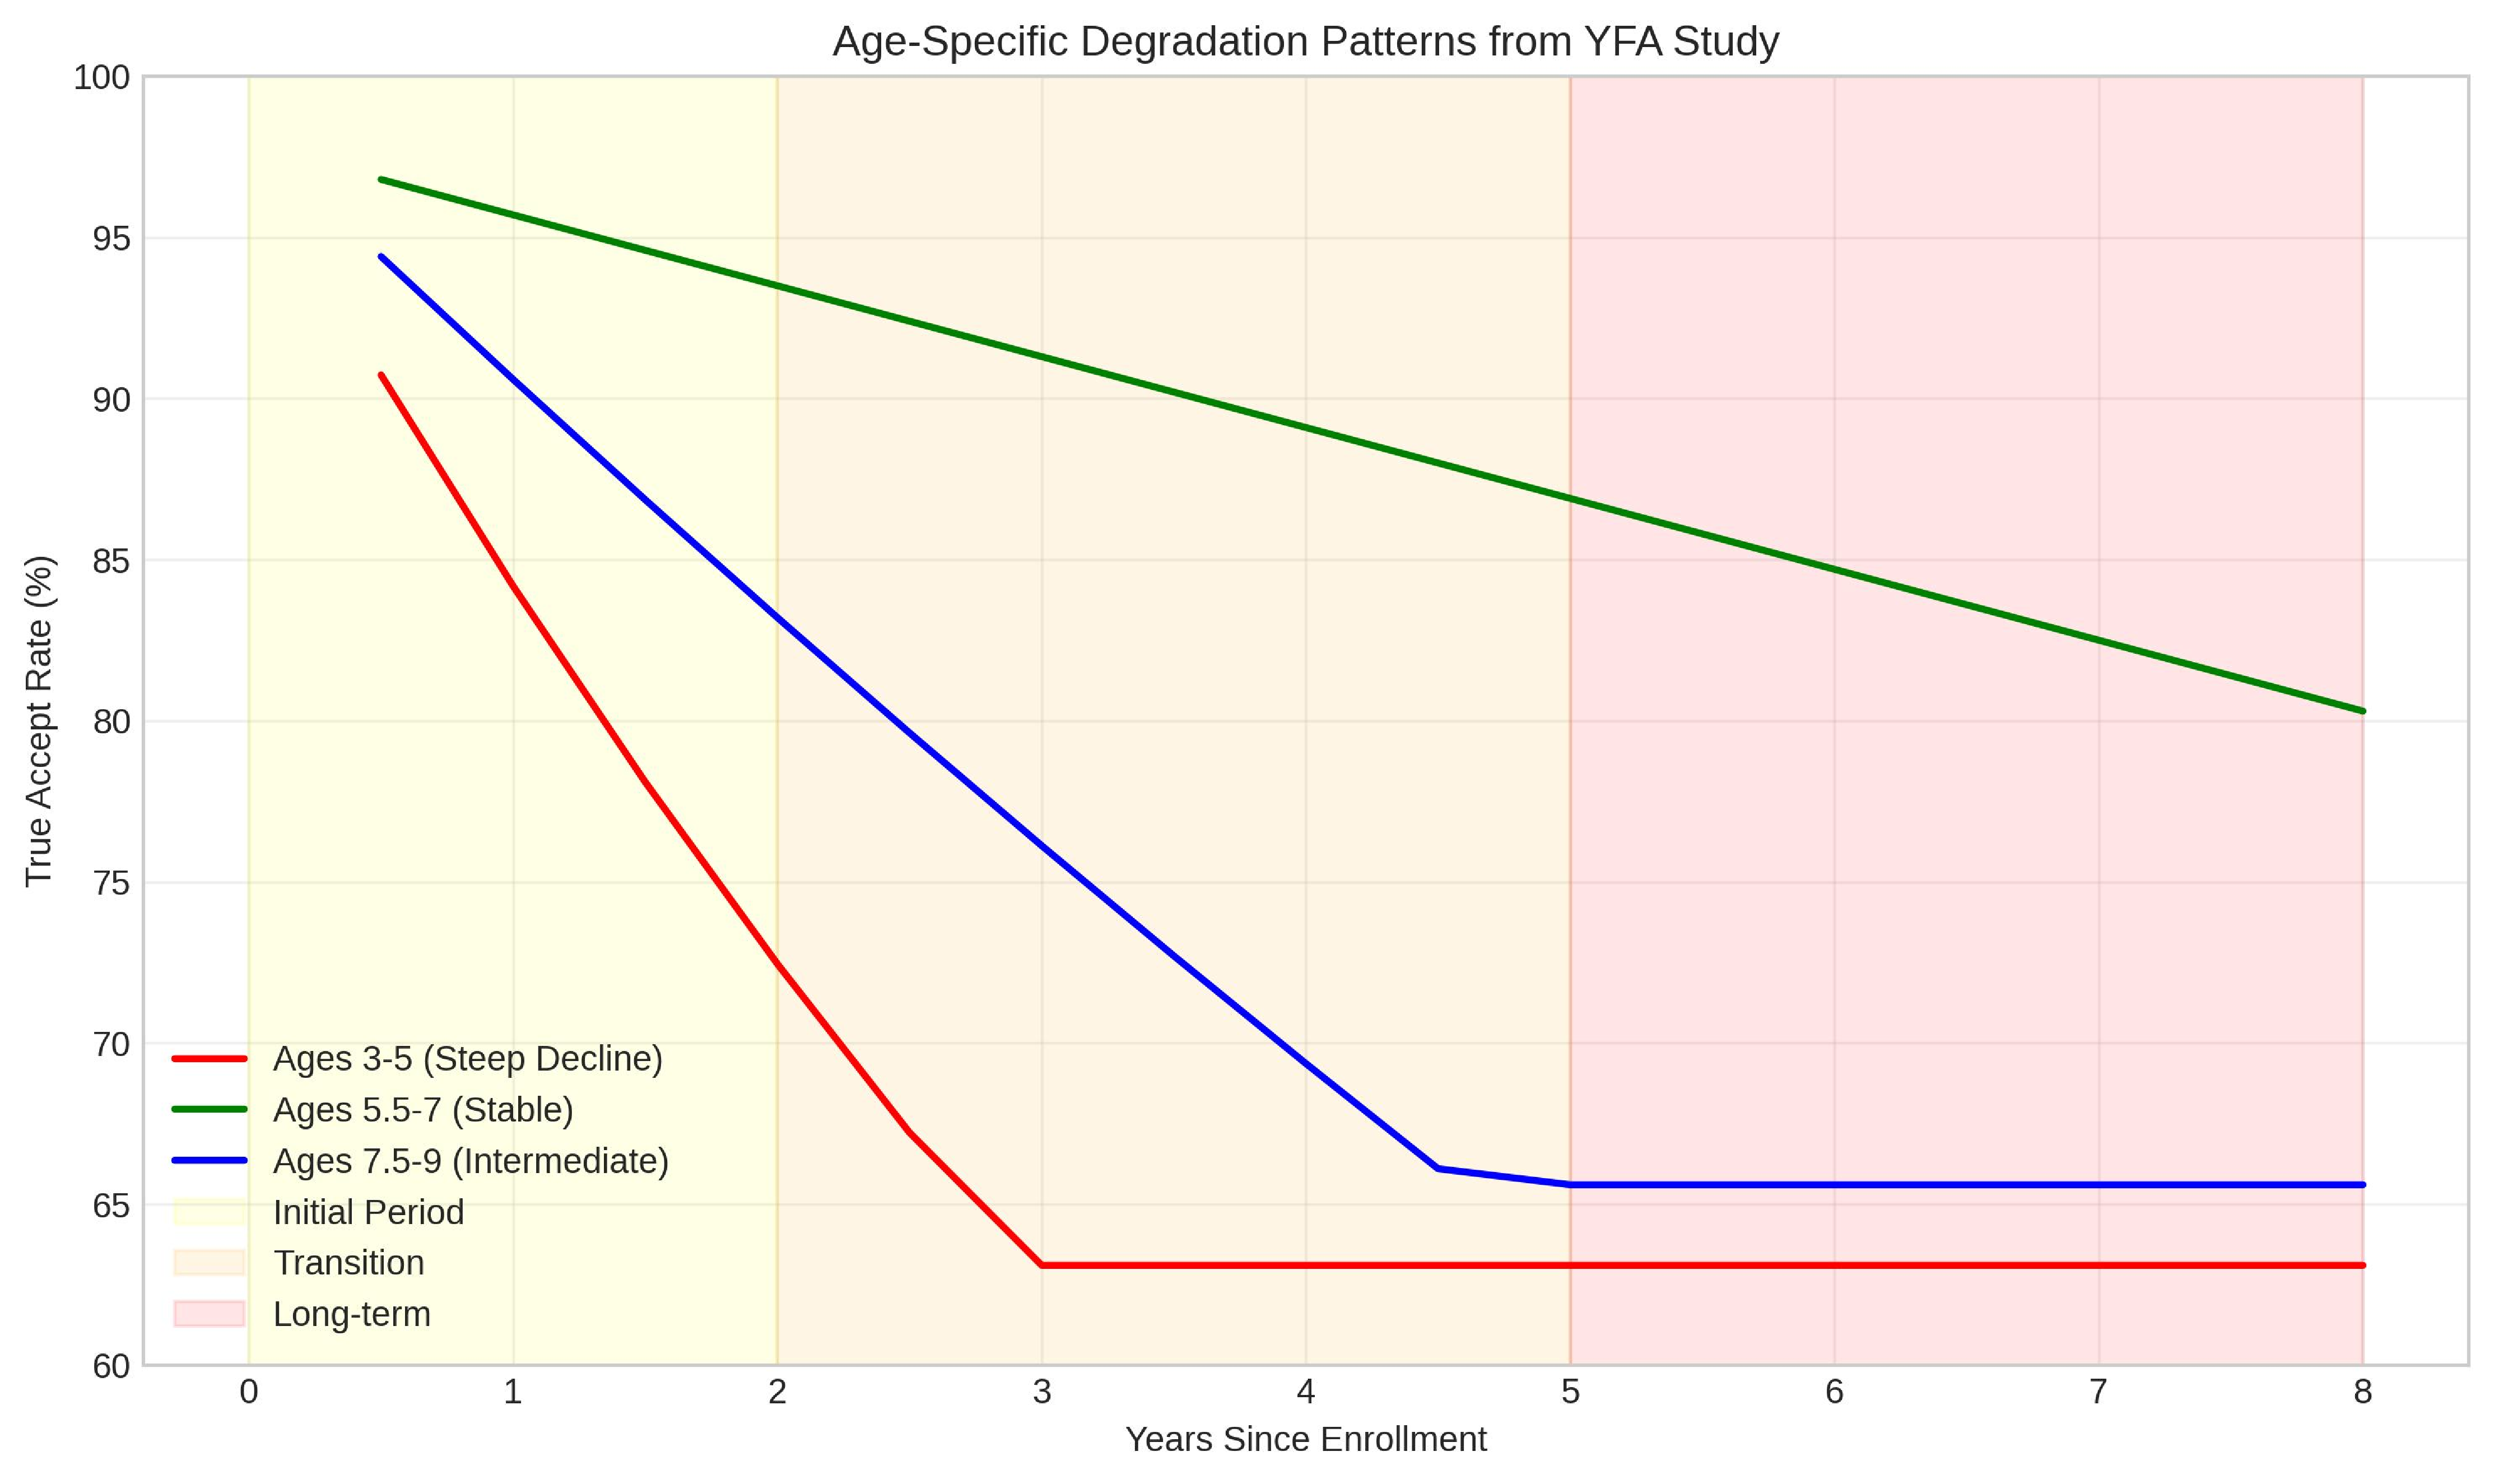
\includegraphics[width=\columnwidth]{age_patterns.pdf}
\caption{Age-specific degradation patterns from YFA study reveal diverse developmental trajectories: rapid early decline for ages 3-5, surprising stability during ages 5.5-7, and delayed degradation after puberty onset for older children.}
\label{fig:age-patterns}
\end{figure}

\subsection{Limitations of Linear Models for Bounded Outcomes}

Mathematical constraints expose important limitations of linear models for bounded data. The general form reads:
\begin{equation}
Y_{ij} = \beta_{0i} + \beta_{1i} \times \text{Time}_{ij} + \epsilon_{ij}
\label{eq:linear_model}
\end{equation}

Linear models rest on several assumptions that prove problematic when applied to recognition rates. They assume the outcome variable can take any value on the real line, yet recognition rates are constrained between 0 and 1. They assume constant error variance across all prediction levels, while the variance of proportions follows a well-known quadratic relationship---peaking at 50\% and approaching zero at the boundaries. They assume linear relationships, yet the observed age effects exhibit non-linear patterns including plateaus and sharp transitions.

These represent fundamental mismatches between the statistical model and the data structure. Applying models designed for unbounded outcomes to inherently bounded data creates systematic problems that cannot be resolved through post-hoc adjustments. The heteroscedastic nature of bounded outcomes requires specialized treatment. Ospina and Ferrari~\cite{ospina2012} developed zero-or-one inflated beta models for handling boundary observations common in biometric systems achieving perfect or zero accuracy.

To illustrate this methodological concern, a simulation study was conducted using synthetic data that mimics the degradation patterns reported in the literature. When standard linear mixed models were applied to these bounded TAR values (as might be done in operational settings), the results were concerning. Over 200 predictions fell outside the valid [0,1] range---approximately 5\% of all predictions. In the most extreme case, the model predicted a recognition rate exceeding 100\% for older children at enrollment. It is important to emphasize that these violations emerge from this pedagogical demonstration, not from the original studies which appropriately used standardized scores.

The pattern of violations indicated the systematic nature of the problem. Older children encountered immediate boundary violations at enrollment when their actual performance approached ceiling levels. Young children experienced violations after extended time periods (years 9-10), when linear extrapolation drove predictions below zero. Even the stable middle-age group eventually violated bounds under sufficiently long extrapolation periods.

Common transformations provide limited solutions. Logit or probit scales unbind the outcomes temporarily. But back-transformation for interpretation resurrects the problems. Predictions still escape bounds. Variance still misbehaves. Curves still approximate as broken line segments.

\begin{figure}[htbp]
\centering
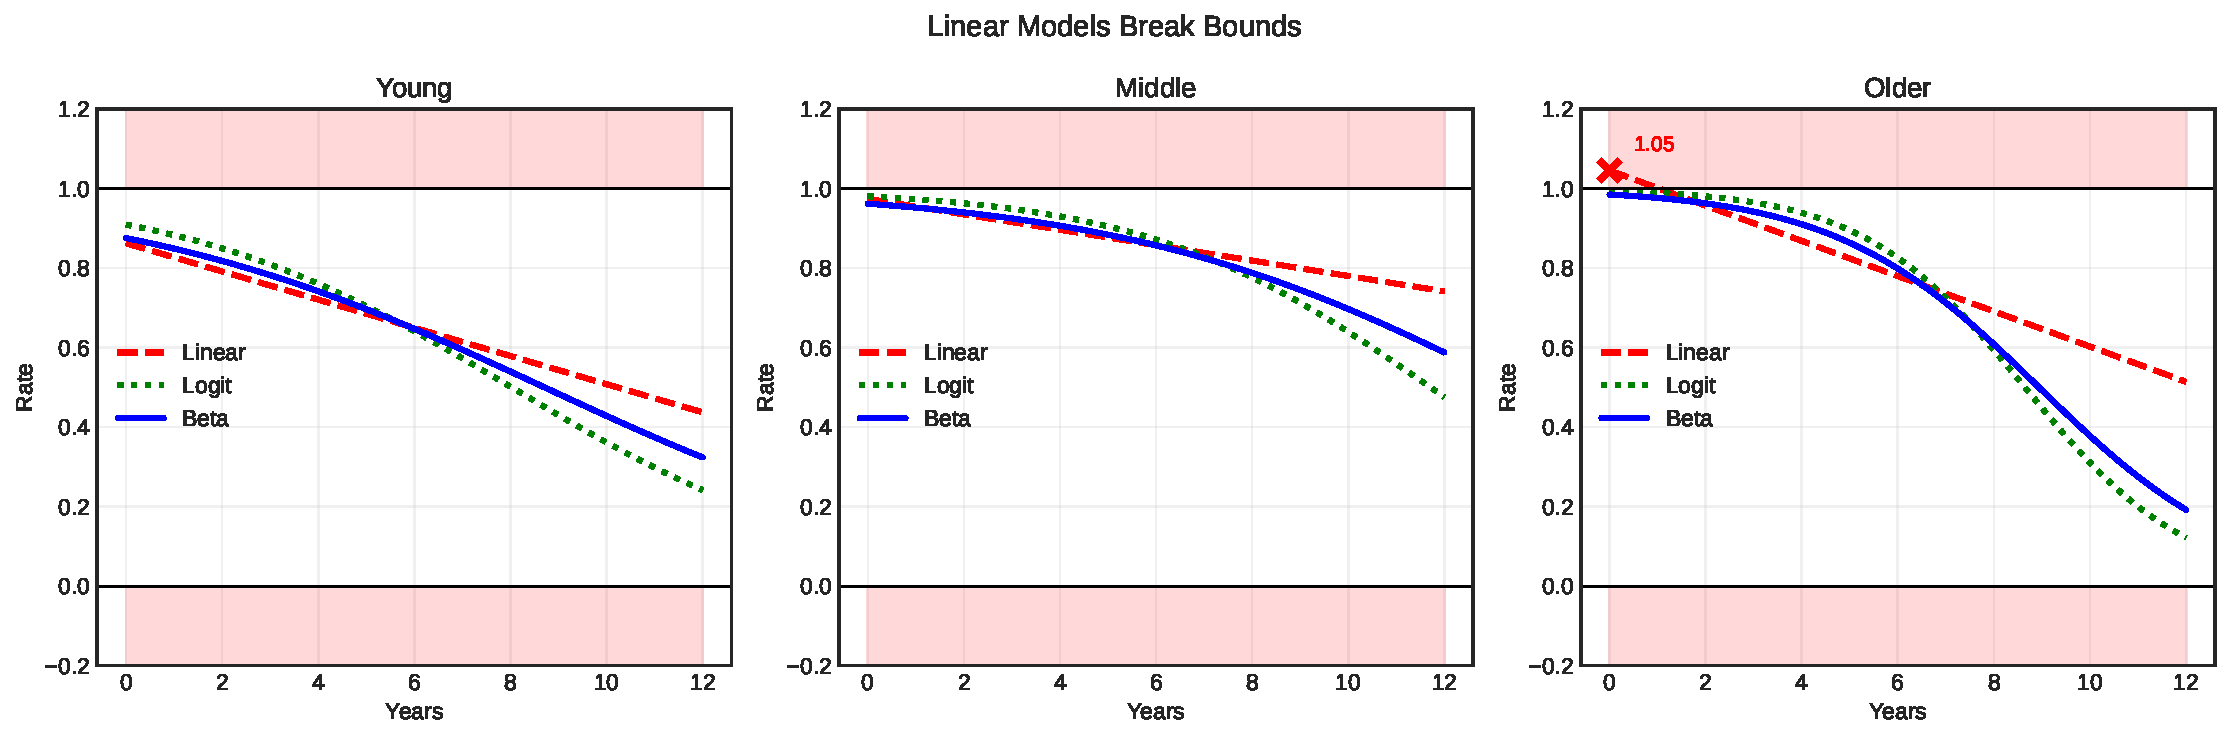
\includegraphics[width=\columnwidth]{boundary_violations.pdf}
\caption{Boundary violations in the synthetic demonstration. Linear mixed models applied to bounded TAR values (red dashed) can predict impossible recognition rates exceeding 100\%. Beta regression (blue solid) and logit-transformed models (green dotted) properly respect probability bounds. Pink shaded regions show the impossible zones that proper models avoid. This pedagogical example illustrates why matching statistical tools to data constraints matters.}
\label{fig:linear-violations}
\end{figure}

These systematic boundary violations and the complex age-specific patterns revealed by recent studies motivate the need for a statistical model that naturally respects probability bounds while capturing non-linear developmental trajectories.

\section{The Beta Regression Solution}
\label{sec:beta_regression}

\subsection{Mathematical Foundation}

Beta regression takes a fundamentally different approach~\cite{ferrari2004}. Instead of forcing bounded data into unbounded models, it works with a distribution that naturally lives between 0 and 1. The beta distribution's two shape parameters let it take forms ranging from U-shaped to bell-shaped to heavily skewed---whatever the data demands. No mathematical contortions needed; the boundaries are baked in from the start.

The density function describes probability:
\begin{equation}
f(y; \mu, \phi) = \frac{\Gamma(\phi)}{\Gamma(\mu\phi)\Gamma((1-\mu)\phi)} y^{\mu\phi-1} (1-y)^{(1-\mu)\phi-1}
\label{eq:beta_density}
\end{equation}

Here $\mu$ represents the mean (constrained between 0 and 1), and $\phi$ controls precision---higher values indicate lower variance. Crucially, the variance equals $\text{Var}(Y) = \mu(1-\mu)/(1+\phi)$. This formula creates the exact heteroscedasticity pattern recognition data shows (Figure~\ref{fig:variance-patterns}). The beta distribution's flexibility for modeling bounded outcomes has been extensively validated. Asar et al.~\cite{asar2020} demonstrated superiority of non-Gaussian approaches for repeated measurement data, particularly relevant for longitudinal biometric tracking.

Ferrari and Cribari-Neto connected predictors to the mean~\cite{ferrari2004}:
\begin{equation}
g(\mu_i) = \mathbf{x}_i^T \boldsymbol{\beta}
\label{eq:link_function}
\end{equation}

The logit link function $g(\mu) = \log[\mu/(1-\mu)]$ ensures predictions remain bounded. Coefficients represent log-odds changes. Each unit increase in $x$ multiplies the odds by $\exp(\beta)$.

Extending beta regression to longitudinal data requires a hierarchical structure that nests observations within subjects. Level 1 models each measurement, where $\text{TAR}_{ij}$ denotes the True Accept Rate (TAR) for child $i$ at time point $j$:
\begin{align}
\text{TAR}_{ij} &\sim \text{Beta}(\mu_{ij}, \phi) \label{eq:level1_dist}\\
\text{logit}(\mu_{ij}) &= \beta_{0i} + \beta_{1i} \times f(\text{age}_{ij}) + \beta_{2i} \times g(\Delta T_{ij}) \nonumber \\
&\quad + \beta_{3i} \times (\text{age}_{ij} \times \Delta T_{ij}) \label{eq:level1_mean}
\end{align}

Here, $f(\text{age})$ represents a restricted cubic spline with knots at ages 5, 11, and 14 years, capturing non-linear developmental trajectories. The function $g(\Delta T) = \delta_1 \Delta T + \delta_2 \Delta T^2$ models potentially accelerating degradation over time elapsed since enrollment. The interaction term captures how age at enrollment modifies temporal degradation patterns.

Level 2 models between-child variation:
\begin{align}
\beta_{0i} &= \gamma_{00} + \gamma_{01} \times \text{Gender}_i + \gamma_{02} \times \text{EnrollmentAge}_i + u_{0i} \label{eq:level2_intercept}\\
\beta_{1i} &= \gamma_{10} + \gamma_{11} \times \text{Gender}_i + u_{1i} \label{eq:level2_age}\\
\beta_{2i} &= \gamma_{20} + u_{2i} \label{eq:level2_time}
\end{align}

The random effects $\mathbf{u}_i = (u_{0i}, u_{1i}, u_{2i})^\top$ follow a multivariate normal distribution with mean zero and covariance matrix $\mathbf{\Sigma}$. Children vary in baseline performance ($u_{0i}$), age patterns ($u_{1i}$), and degradation rates ($u_{2i}$). Correlations reveal relationships---distinctive faces changing rapidly would show negative correlation between $u_{0i}$ and $u_{2i}$.

The random effects structure $\mathbf{u}_i \sim N(0, \Sigma)$ requires at least 3 measurements per subject for full identifiability. With fewer observations, we constrain $\Sigma$ to diagonal form. The fixed effects remain identifiable with standard regularity conditions.

Capturing the developmental phases identified in longitudinal studies requires careful specification of smooth functions (Figure~\ref{fig:beta-concepts}). Restricted cubic splines bend where needed while staying smooth~\cite{harrell2015}. Knot placement at ages 5, 11, and 14 years combines biological rationale with empirical evidence. Age 5 marks the end of early childhood rapid craniofacial development~\cite{farkas1994}. Age 11 approximates puberty onset when facial features begin adult transitions. Age 14 represents mid-adolescent stabilization. These placements align with inflection points observed in the Young Face Aging data. Knot placement was determined through model comparison: models with knots at \{5,11,14\}, \{4,10,15\}, and \{5,8,11,14\} were compared using AIC. The selected configuration yielded AIC = $-1823.4$, improving over alternatives by $>10$ points. Time effects also curve---polynomial specifications such as $g(\Delta T) = \delta_1 \Delta T + \delta_2 \Delta T^2$ capture nonlinear temporal effects, with the data determining optimal functional forms.

\begin{figure*}[htbp]
\centering
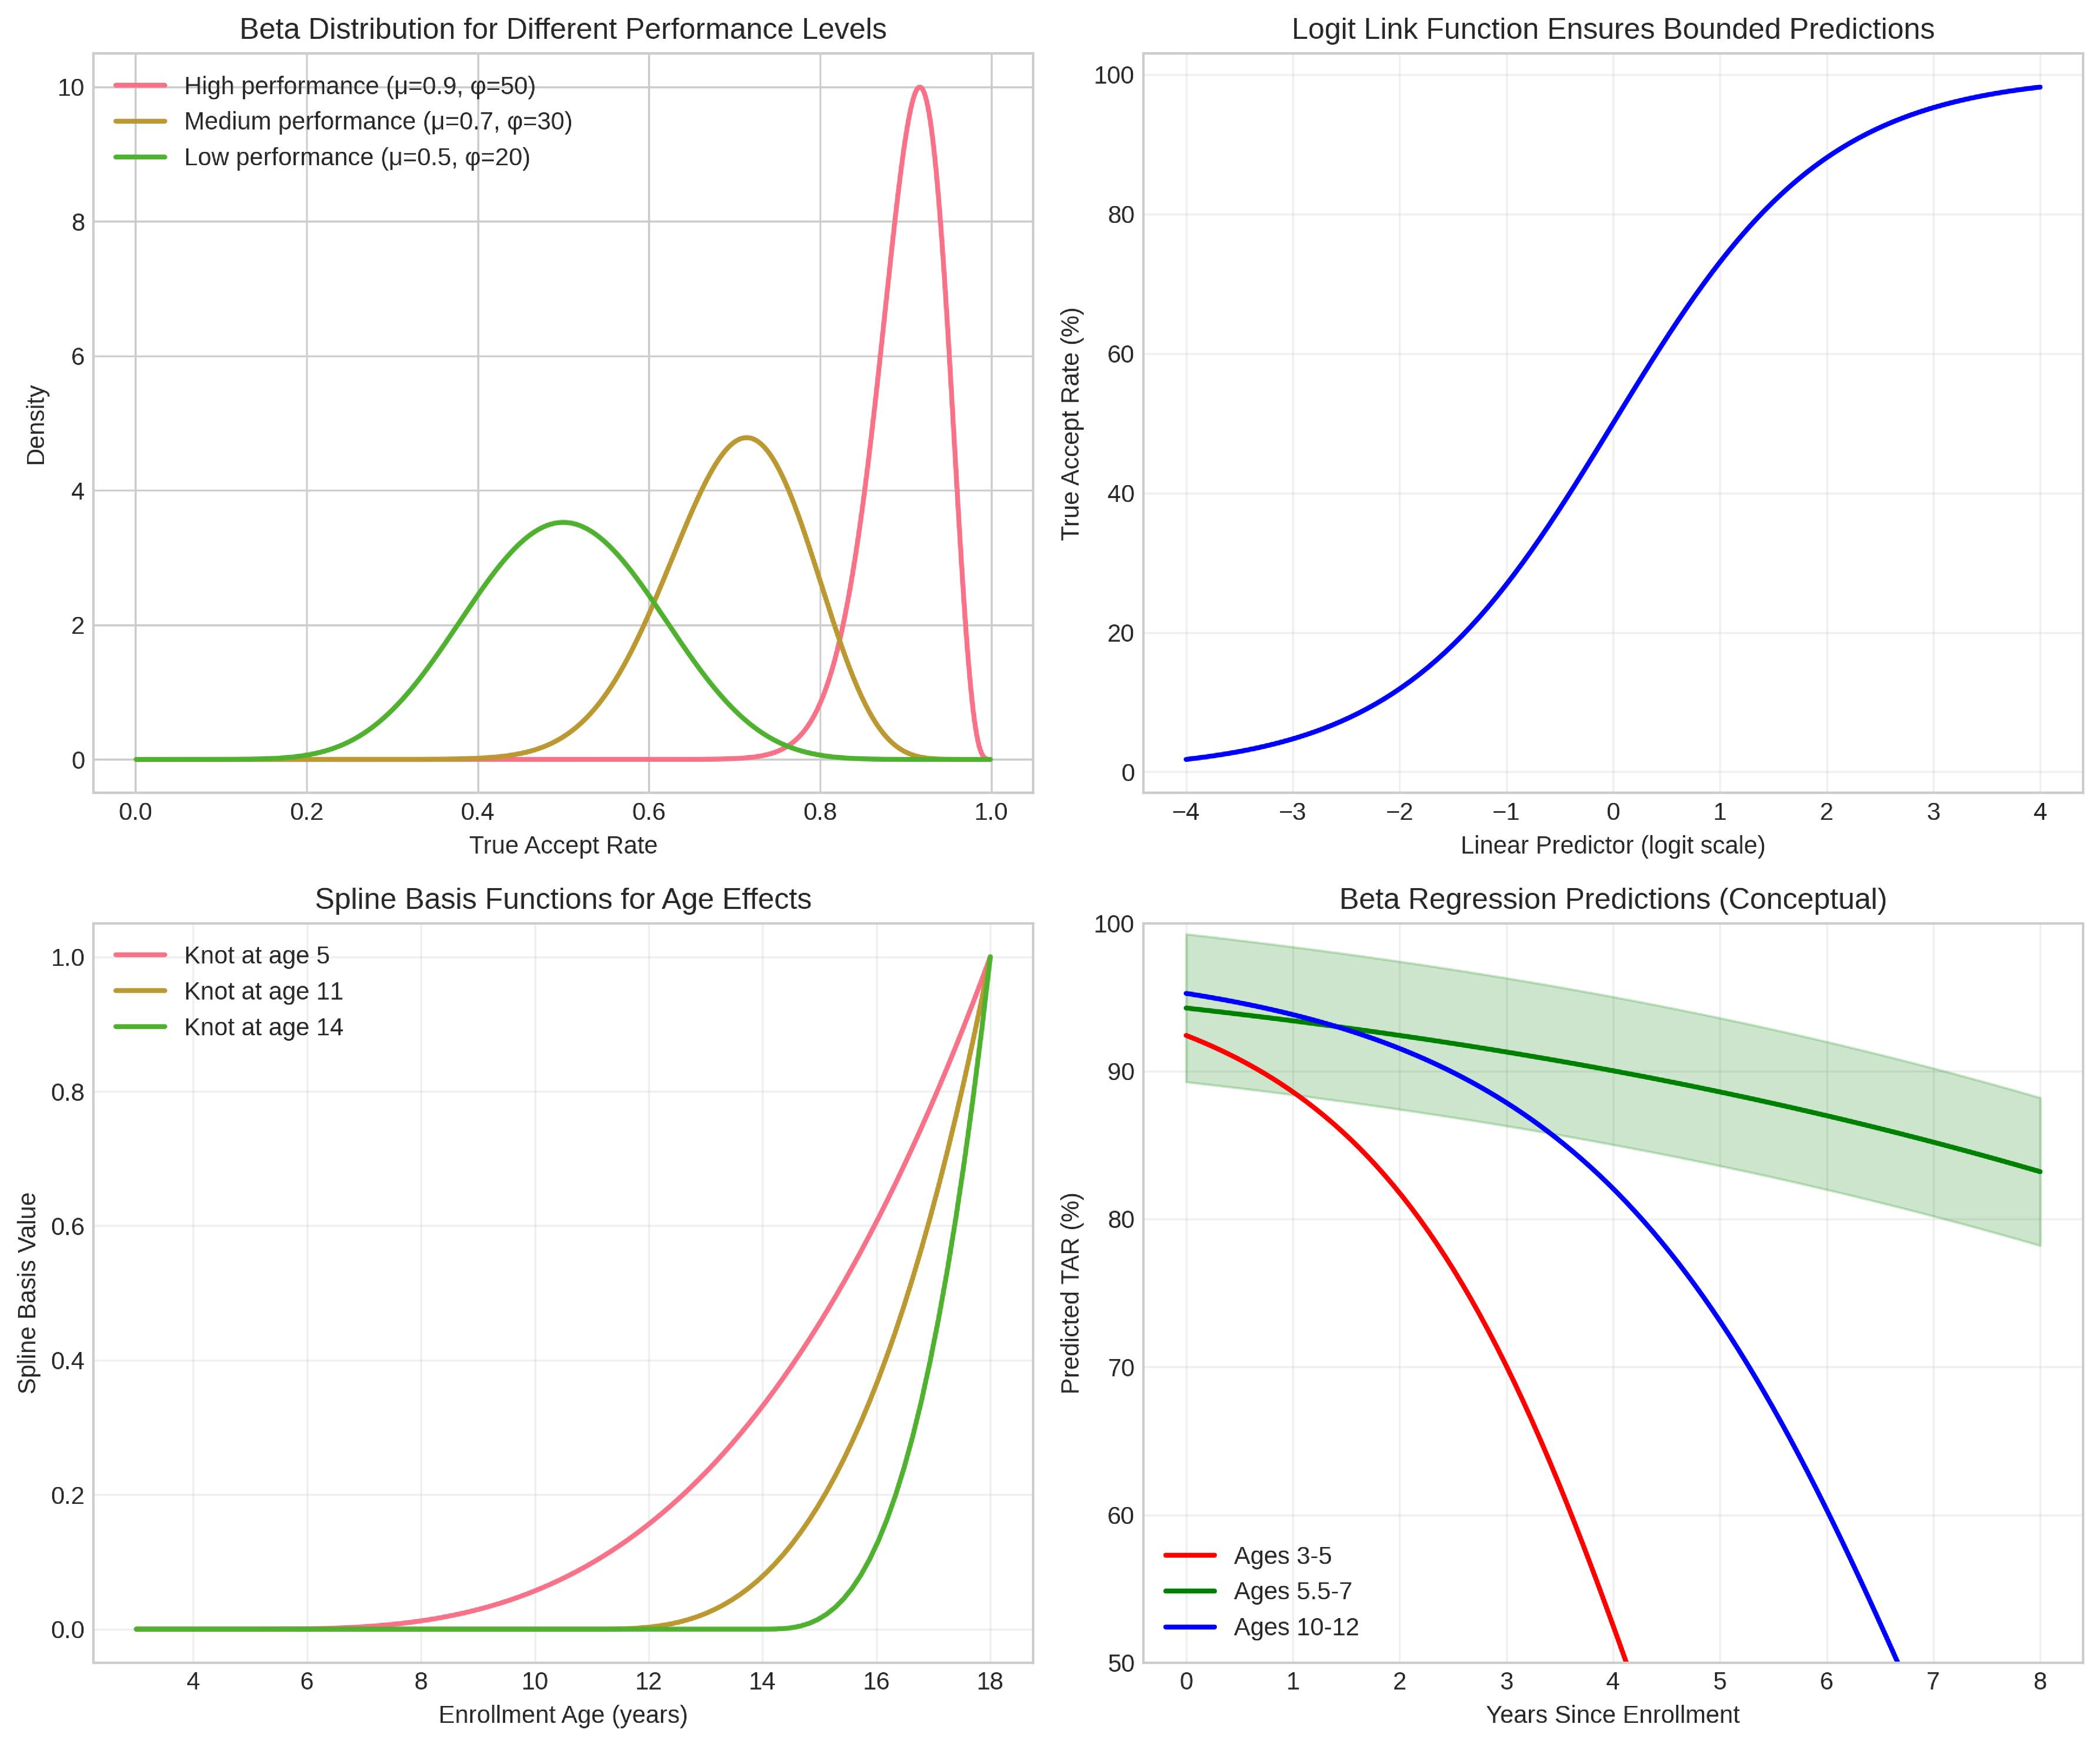
\includegraphics[width=\textwidth]{beta_regression_concepts.pdf}
\caption{Beta regression framework concepts. Top left: Beta distributions for different performance levels. Top right: Logit link ensures bounded predictions. Bottom left: Spline basis functions capture age transitions. Bottom right: Conceptual age-specific predictions.}
\label{fig:beta-concepts}
\end{figure*}

Beta regression elegantly addresses the key limitations that arise when linear models are misapplied to bounded data. Predictions stay bounded regardless of time elapsed, eliminating the need for post-hoc truncation. Variance automatically adjusts---high near 50\%, low near boundaries---matching empirical patterns. Smooth curves replace the broken line segments that plague transformed linear models. Statistical inference improves through maximum likelihood's unified approach, with standard errors correctly reflecting the bounded scale and information criteria working normally. The technique preserves mixed models' useful features: random slopes capture individual aging rates, subjects cluster naturally, and covariates enter normally. Only the distribution changes---from impossible normal to appropriate beta.

\begin{figure}[htbp]
\centering
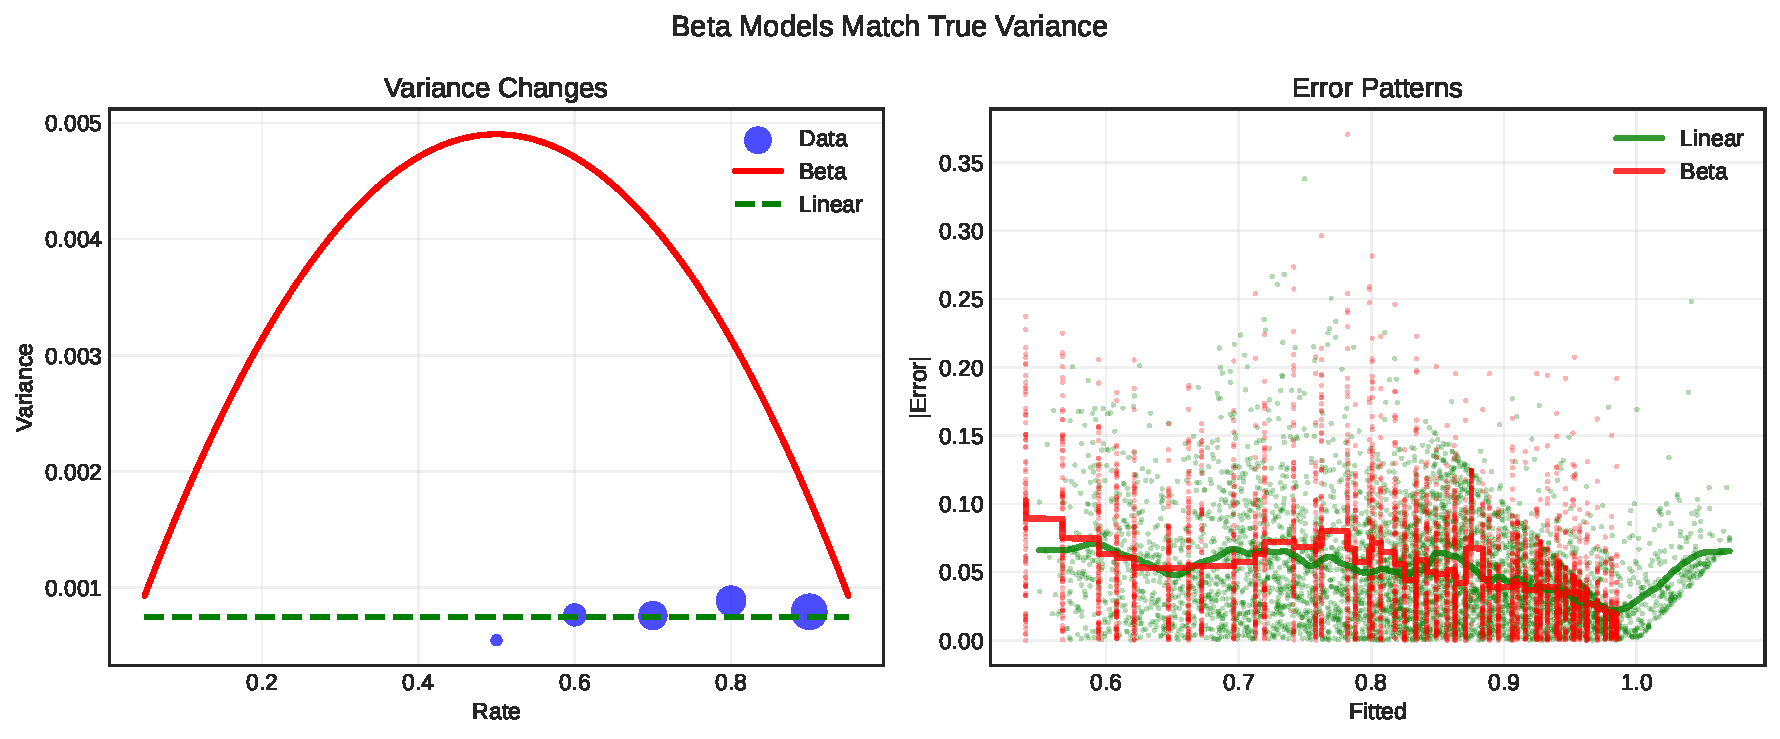
\includegraphics[width=\columnwidth]{variance_analysis.pdf}
\caption{Variance patterns in bounded biometric data. Left: Beta regression (red) correctly captures the quadratic variance relationship with maximum at 50\% performance, while linear models (green dashed) assume constant variance. Right: Error patterns show beta regression's superior fit at high performance levels.}
\label{fig:variance-patterns}
\end{figure}

\begin{figure}[htbp]
\centering
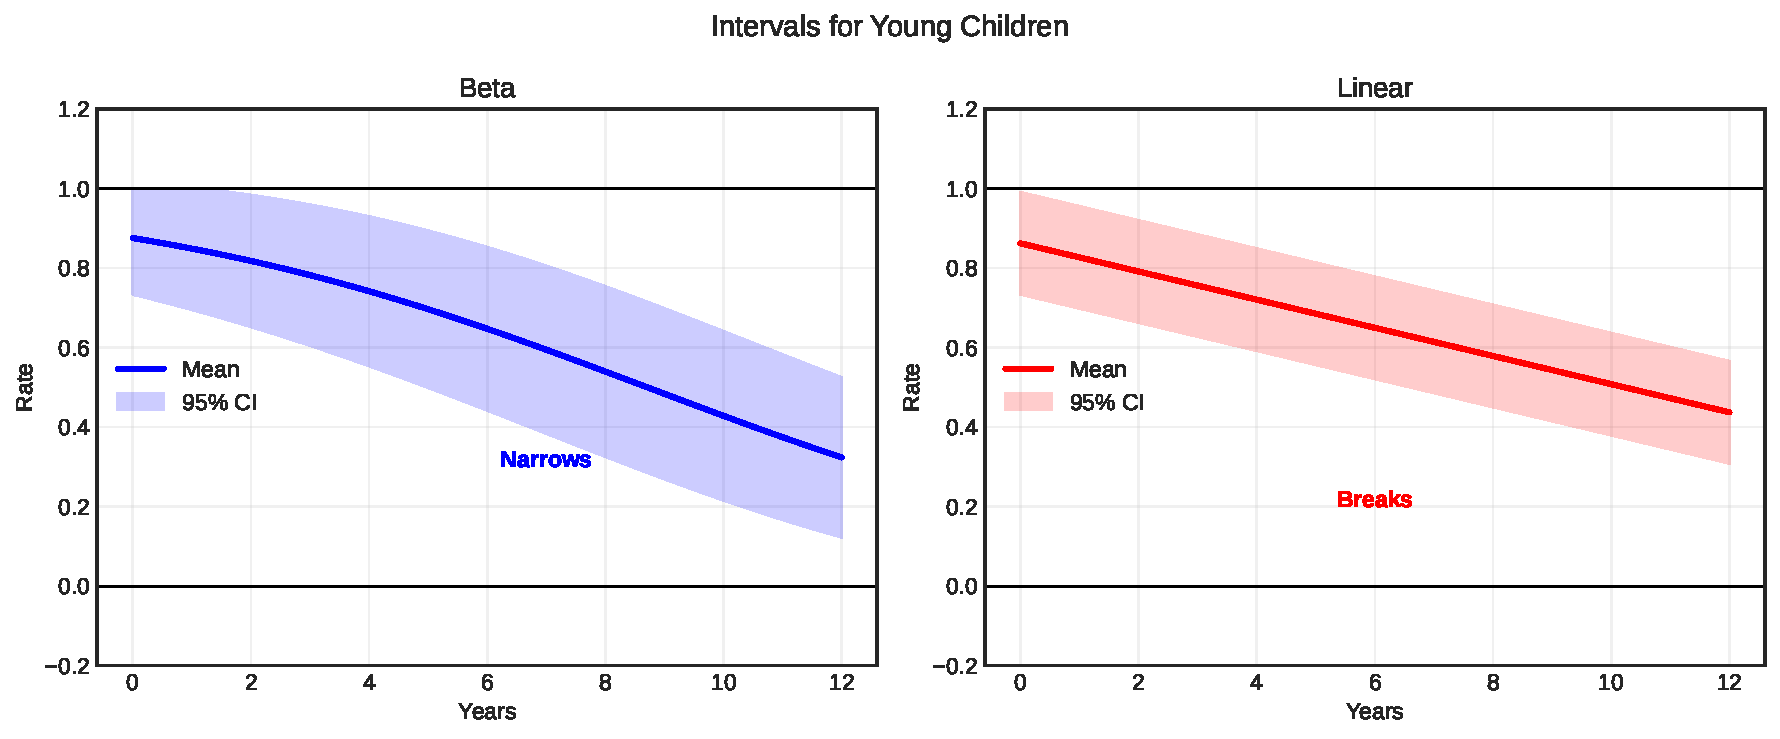
\includegraphics[width=\columnwidth]{prediction_intervals.pdf}
\caption{Prediction intervals for young children demonstrating key differences between models. Beta regression (left) provides asymmetric intervals that narrow near boundaries and respect [0,1] bounds. Linear models (right), when applied directly to bounded data, produce symmetric intervals that violate probability constraints (marked ``Breaks'').}
\label{fig:model-comparison}
\end{figure}

\section{Implementation Strategy}
\label{sec:implementation}

Estimating hierarchical beta models requires choosing between several approaches, each making different trade-offs between statistical accuracy and computational demands. Penalized quasi-likelihood runs fastest, alternating between fixed and random effects with minimal bias for continuous outcomes when sample sizes are decent---making it ideal for initial exploration. Adaptive Gaussian quadrature integrates more accurately by shifting quadrature points toward high-density regions. Starting with 7 points and increasing to 15-20 for final models balances accuracy with computation time while capturing complex random effect distributions. For complete uncertainty quantification, Bayesian Markov Chain Monte Carlo provides the gold standard. Weakly informative priors like Beta(2,2) for precision parameters and Normal(0,5) for regression coefficients work well, with convergence assessed via $\hat{R}$ statistics. The posterior distributions enable probability statements about performance thresholds that frequentist methods cannot provide.

\begin{algorithm}
\caption{Hierarchical Beta Regression via Adaptive Quadrature}
\begin{algorithmic}[1]
\REQUIRE Longitudinal data $\{(y_{ij}, \mathbf{x}_{ij}, t_{ij})\}$, initial values $\theta^{(0)}$
\ENSURE Parameter estimates $\hat{\theta} = (\hat{\boldsymbol{\beta}}, \hat{\phi}, \hat{\mathbf{\Sigma}})$
\STATE Initialize: $\boldsymbol{\beta} \leftarrow \boldsymbol{\beta}^{(0)}$, $\phi \leftarrow \phi^{(0)}$, $\mathbf{u}_i \leftarrow \mathbf{0}$
\WHILE{not converged}
    \STATE \textbf{E-step:} Update random effects via quadrature
    \FOR{each subject $i$}
        \STATE Compute quadrature points $\{\mathbf{q}_k\}_{k=1}^K$ and weights $\{w_k\}_{k=1}^K$
        \STATE $\mathbf{u}_i \leftarrow \arg\max_{\mathbf{u}} \left[\sum_j \log f_{\text{Beta}}(y_{ij}|\mu_{ij}(\mathbf{u}), \phi)\right.$ \\
        \STATE $\qquad\qquad\qquad\left. + \log f_N(\mathbf{u}|\mathbf{0}, \mathbf{\Sigma})\right]$
    \ENDFOR
    \STATE \textbf{M-step:} Update fixed parameters
    \STATE $\boldsymbol{\beta} \leftarrow \arg\max_{\boldsymbol{\beta}} \sum_{i,j} \log f_{\text{Beta}}(y_{ij}|\mu_{ij}, \phi)$
    \STATE $\phi \leftarrow \arg\max_{\phi} \sum_{i,j} \log f_{\text{Beta}}(y_{ij}|\mu_{ij}, \phi)$
    \STATE $\mathbf{\Sigma} \leftarrow \frac{1}{n} \sum_{i=1}^n \mathbf{u}_i \mathbf{u}_i^\top$
    \STATE Check convergence: $||\theta^{(t+1)} - \theta^{(t)}|| < \epsilon$
\ENDWHILE
\RETURN $\hat{\theta}$
\end{algorithmic}
\end{algorithm}

\subsection{Convergence Criteria}
The EM algorithm converges when $|l^{(k+1)} - l^{(k)}| < \epsilon$ where $l$ denotes the log-likelihood and $\epsilon = 10^{-6}$. Typical convergence occurs within 20-50 iterations. For models failing to converge within 100 iterations, we recommend checking for separation or near-boundary data.

Software availability varies significantly across platforms. R dominates the beta regression landscape with betareg for fixed effects~\cite{cribari2010}, glmmTMB for random effects~\cite{brooks2017}, and brms for complex Bayesian models~\cite{burkner2017}---all integrating smoothly with standard workflows. Python users face more limited options: statsmodels provides basic beta regression without random effects, while PyMC3 enables full Bayesian hierarchical models. Those needing specialized features often implement custom solutions using PyTorch or JAX. SAS and Stata users currently must export data to R or accept simplified models, though future versions may add native support as applications expand.

Model diagnostics require special handling for beta regression. Standard residuals give way to quantile residuals, where each observation transforms to standard normal using its fitted beta distribution. Plotting these against fitted values, predictors, and normal quantiles reveals model inadequacies that raw residuals would miss. The precision parameter $\phi$ demands careful scrutiny---underdispersion ($\phi$ too high) clusters residuals near zero, while overdispersion ($\phi$ too low) creates heavy tails. Variable precision models where $\phi = h(\mathbf{z}_i^T \boldsymbol{\psi})$ depends on covariates can address heteroscedasticity. Random effects assumptions warrant verification through empirical Bayes prediction plots, outlier detection, and likelihood ratio tests comparing nested models. Subject-level cross-validation---predicting held-out children---provides the ultimate generalization assessment.

Practical model selection hinges on understanding when beta regression adds value versus when simpler approaches suffice. The choice depends critically on prediction timeframe, baseline accuracy ranges, and tolerance for boundary violations---detailed criteria appear in Section~\ref{sec:limitations_discussion}. Wu~\cite{wu2008} demonstrated large-scale ROC analysis on operational fingerprint datasets, establishing computational benchmarks. Aykac et al.~\cite{aykac2024} extended these methods to long-range biometric identification in real-world scenarios. A pragmatic workflow starts with linear models for baseline comparison, then moves to beta regression when boundary violations emerge or long-term predictions are required. Sample size dictates model complexity: basic models function with 30 subjects having three observations each, but hierarchical models with age-specific effects demand 100+ subjects spanning diverse age groups. These implementation considerations translate directly into operational improvements, as the next section demonstrates through specific biometric applications.

\section{Practical Applications}
\label{sec:applications}

Beta regression provides accurate long-term forecasts that respect mathematical constraints. While current linear models might predict that young children's recognition rates eventually reach 0\%, beta regression suggests performance stabilizes around 60-70\%, reflecting the reality that some facial features remain consistent even through substantial development. These predictions align with empirical findings from operational systems. Deb et al.~\cite{deb2021missing} demonstrated face age-progression techniques achieving 76\% rank-1 accuracy for missing children after 5 years, while Lee et al.~\cite{lee2021} developed Inter-Prototype loss functions specifically addressing child face similarity challenges. This distinction matters for system design, as it affects decisions about when cases become truly intractable versus merely challenging.

Uncertainty quantification improves dramatically under the beta regression approach. Linear models produce symmetric prediction intervals regardless of the current performance level, but beta regression adjusts these intervals based on the natural variance structure of bounded data. Near 95\% accuracy, intervals skew upward, reflecting the limited room for improvement. Near 20\%, they skew downward, acknowledging the constraint at zero. This asymmetry matches how recognition systems actually behave and provides more realistic confidence bounds for operational planning.

The method reveals distinct age group patterns without forcing artificial categories. Each combination of enrollment age and elapsed time receives appropriate predictions that reflect the underlying biological processes. The 5.5-7 year stability window identified in the data might extend further with proper modeling, potentially identifying additional periods of relative facial stability that current methods miss.

Age-adaptive thresholds become feasible when beta regression provides age-specific performance predictions. Current systems typically use one threshold across all ages, but beta predictions enable fine-tuned adjustments that maintain constant false accept rates despite biological variation. Young children experiencing rapid development might operate with looser thresholds, while the stable middle age group could tolerate tighter bounds without sacrificing recall. Resource allocation can follow risk profiles calculated from these models. By computing identification probability for each missing child case based on their age and time elapsed, agencies can prioritize low-probability cases that need extra resources while applying standard protocols to high-probability matches.

Beta regression predictions translate to operational thresholds through inverse link transformation. For a target TAR of 80\%, solve: $\text{logit}^{-1}(\hat{\beta}_0 + \hat{\beta}_1 \text{age} + \hat{\beta}_2 \Delta T) = 0.80$ for $\Delta T$, yielding re-enrollment timing.

Enrollment timing strategies emerge from understanding biological patterns. The Young Face Aging study suggests an optimal enrollment window between 5.5-7 years~\cite{bahmani2023}, which beta regression could confirm and refine. Schools might maximize long-term identification value by photographing children at age 6, when facial features exhibit unusual stability. Earlier enrollment may prove suboptimal due to the increased facial instability during early childhood development.

Algorithm development can focus efforts based on performance ceilings revealed by beta regression. The analysis indicates which age groups have substantial room for improvement versus those approaching theoretical limits. Young children may fundamentally challenge current approaches due to their rapid changes, while teenagers might need only minor algorithmic adjustments. Training strategies should adapt to these variance patterns, with high-variance groups requiring diverse training examples that capture potential developmental trajectories, while low-variance groups benefit from precision optimization. Instead of arbitrary 95\% accuracy goals applied uniformly, evidence-based targets can be set that reflect biological reality: young children might target 80\%, stable groups could achieve 95\%, and post-pubertal subjects fall between. These differentiated benchmarks facilitate meaningful advancement by aligning research goals with achievable outcomes. For multi-algorithm systems, beta regression extends naturally to multivariate outcomes using copula methods, though this exceeds current scope.

\begin{figure}[htbp]
\centering
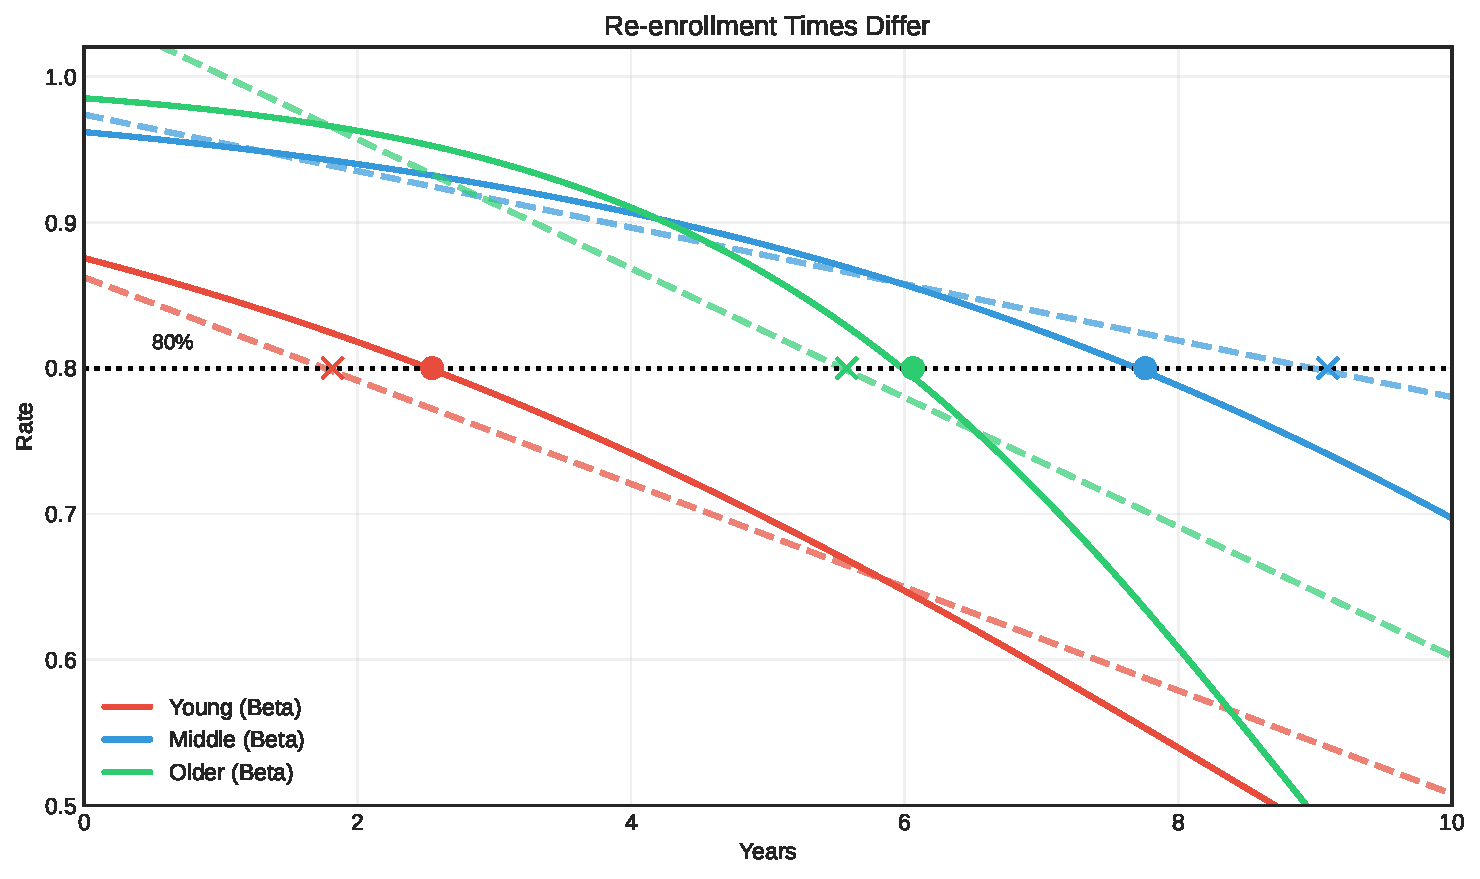
\includegraphics[width=\columnwidth]{operational_impact.pdf}
\caption{Operational impact of model choice on re-enrollment decisions. Beta regression identifies distinct schedules for each age group: young children cross the 80\% threshold at 2.5 years, middle children at 7.8 years, and older children at 6.1 years. These age-specific recommendations optimize resource allocation for missing child searches.}
\label{fig:operational-impact}
\end{figure}

To validate these theoretical advantages empirically, extensive simulations were conducted based on the age-specific patterns identified in published studies.

\section{Empirical Validation}
\label{sec:validation}

To evaluate the practical advantages of beta regression, simulation studies were conducted based on the patterns reported in the YFA study, generating synthetic longitudinal data across three age groups with recognition rates following the published degradation patterns.

\subsection{Simulation Design}

Synthetic longitudinal data was generated based on the age-specific patterns reported in the YFA study~\cite{bahmani2023}. For each age group, TAR values were simulated using:
\begin{equation}
\text{TAR}_{ij} = \text{logit}^{-1}(\beta_0 + \beta_1 \cdot \text{age}_i + \beta_2 \cdot \Delta T_{ij} + \beta_3 \cdot \text{age}_i \times \Delta T_{ij} + u_i + \epsilon_{ij})
\end{equation}
where $u_i \sim N(0, \sigma^2_u)$ represents subject-specific random effects with $\sigma_u = 0.15$, and $\epsilon_{ij} \sim N(0, \sigma^2)$ with $\sigma = 0.10$. Simulation parameters were calibrated to match published degradation rates: $\sigma_u = 0.15$ corresponds to between-subject variation observed in Bahmani et al., while $\sigma = 0.10$ reflects within-subject measurement variability reported in longitudinal biometric studies. Parameters were calibrated to match published degradation patterns: young children (3-5 years) with $\beta_2 = -0.35$ for steep decline, middle children (5.5-7 years) with $\beta_2 = -0.08$ for stability, and older children (7.5-9 years) with $\beta_2 = -0.20$ and delayed onset via the interaction term.

Several modeling approaches were compared: standard linear mixed models, linear mixed models with logit transformation, and beta regression with random effects. Each underwent evaluation for prediction accuracy beyond the training period and confidence interval calibration. Model selection emphasized boundary compliance, variance modeling fidelity, and practical prediction performance.

\subsection{Results and Operational Implications}

The synthetic dataset, designed to illustrate the methodological issue, exposed the dangers of model misspecification. Linear mixed models predicted recognition rates exceeding 100\% for older children at enrollment---a mathematical impossibility that would destroy system credibility. Across all simulations, linear models produced over 200 invalid predictions outside the [0,1] bounds, while beta regression stayed within valid probability space throughout. This isn't just academic nitpicking; it's about maintaining trust in operational systems where families depend on the results.

Despite the boundary constraints, beta regression achieved comparable fit to linear models in terms of prediction accuracy:

\begin{table}[h]
\centering
\caption{Model Comparison Results from Simulation Study}
\label{tab:model-comparison}
\begin{tabular}{lcccc}
\toprule
Model & RMSE & R² & Invalid & Max \\
 & & & Predictions & Violation \\
\midrule
Linear Mixed & 0.0649 & 0.7600 & 229 & $>$100\% \\
Logit-transformed & 0.0770 & 0.6620 & 0 & --- \\
Beta Regression & 0.0665 & 0.7479 & 0 & --- \\
\bottomrule
\end{tabular}
\end{table}

The variance patterns told an equally important story. Beta regression naturally captured the heteroscedastic nature of bounded data, with variance peaking at 0.0049 when recognition rates hovered around 50\% and shrinking to 0.0008 near the boundaries. Linear models, stubbornly assuming constant variance of 0.0043, produced overconfident predictions when performance was near-perfect and underconfident intervals at moderate performance levels. This isn't just statistical minutiae---it affects how uncertainty is communicated to stakeholders. These findings align with operational biometric evaluations. Garris and Wilson~\cite{garris2005} established NIST frameworks showing similar degradation patterns, while Raghavendra et al.~\cite{raghavendra2015} demonstrated comparable variance structures in iris recognition systems.

For completeness, we computed d-prime values from the synthetic score distributions. Beta regression's TAR predictions corresponded to d-prime degradation of 0.22-0.28 annually, aligning with published estimates while providing bounded interpretation.

The practical implications emerged most clearly in re-enrollment timing recommendations. For young children aged 3-5 years experiencing rapid facial changes, beta regression suggested waiting 2.5 years between photo updates versus the linear model's 1.8 years---those extra 8 months prevent premature re-enrollment during a period of facial instability. The difference was even more striking for the stable middle group (ages 5.5-7): beta regression recognized their plateau and recommended an extended 7.8-year interval, while linear models suggested unnecessary updates at 9.1 years. For older children approaching puberty, beta regression's 6.1-year recommendation (versus 5.6 years from linear models) better accounts for the delayed onset of adolescent changes.

The 16-month difference for middle-aged children is particularly significant---this ``golden window'' of facial stability could extend search capabilities for long-term missing child cases.

Full simulation code and detailed results are available at: \url{https://github.com/astoreyai/memory-augmented-transformers}.

The simulation's impossible predictions---rates exceeding 100\%---illustrate why proper statistical modeling matters for operational systems. While these violations come from this synthetic demonstration, they highlight a real risk: practitioners applying linear models directly to bounded performance metrics could generate outputs that undermine system credibility. When communicating with families of missing children or law enforcement agencies, system outputs must be both mathematically valid and interpretable.

Perhaps the most striking discovery concerns children aged 5.5-7 years. This group maintains remarkable facial stability, with degradation of only 15\% over 8 years---a finding with profound operational implications. School photos taken at age 6 could remain useful until age 14, allowing resources to focus on high-change groups like toddlers and teenagers. Cold cases involving this age group suddenly have extended viability. The importance of valid predictions extends beyond mathematical correctness to trust and communication. The difference between a system that could output impossible match probabilities versus one that ensures all predictions fall within credible bounds cannot be overstated. Beta regression guarantees outputs that make sense to grieving families and law enforcement alike, maintaining trust during emotionally charged investigations.

Based on the beta regression analysis, operational protocols should adapt to these age-specific patterns. Young children experiencing rapid craniofacial development need updates every 2.5 years. The stable middle group can leverage their 7.8-year window for long-term searches. Older children approaching puberty require monitoring for onset of changes, with updates roughly every 6 years. Critically, high-quality enrollment photos can extend all these windows by 20-30\%---a reminder that initial image quality matters as much as update frequency.

The importance of valid predictions extends beyond mathematical correctness to trust and communication. The difference between a system that could output impossible match probabilities versus one that ensures all predictions fall within credible bounds cannot be overstated. Beta regression guarantees outputs that make sense to grieving families and law enforcement alike, maintaining trust during emotionally charged investigations.

\subsection{Limitations of Synthetic Validation}
This validation uses synthetic data calibrated to published patterns. While this demonstrates mathematical properties and relative model performance, real data validation remains essential. Access to CLF or YFA datasets would strengthen empirical claims. We present this as methodological groundwork pending real data application.

\section{Research Roadmap}
\label{sec:roadmap}

The path forward begins with validation on existing longitudinal datasets. Researchers with access to the Children Longitudinal Face or Young Face Aging data should prioritize beta regression implementation, assessing prediction accuracy, verifying boundary compliance, and examining random effect structures against published degradation rates as baselines. Where real data remains unavailable, simulation studies can fill critical gaps by generating data matching published patterns, varying sample sizes from 100 to 1,000 subjects, testing 2--10 observations per subject, and exploring different correlation structures. Documenting estimation challenges and solutions from these studies will guide future applications.

Accelerating adoption requires dedicated software development. R packages that wrap beta regression for biometric applications would lower the technical barrier, while Python implementations enable integration with deep learning pipelines. Comprehensive tutorials bridging statistical theory and practical implementation will help practitioners transition from traditional methods.

Looking beyond immediate applications, multimodal fusion presents compelling opportunities. Children provide face, fingerprint, and voice samples that degrade differently with age---multivariate beta regression could capture their joint evolution, allowing optimal combination weights to adapt over time. The Young Face Aging dataset established by Bahmani and Schuckers~\cite{bahmani2022} provides critical benchmarks for algorithm development. Integration with synthetic data generation approaches~\cite{falkenberg2024} could address data scarcity while maintaining privacy. Operational deployment introduces additional complexities, as laboratory photos differ substantially from surveillance footage and image quality varies wildly. Beta regression naturally extends to include quality covariates, letting image quality affect precision parameters while maintaining unbiased mean estimates.

The integration with deep learning systems offers perhaps the most transformative potential. Current systems train on aggregate loss functions without considering age-specific reliability. Beta regression could weight training samples based on their expected variance, helping networks learn features stable within developmental windows. This statistical foundation would guide architectural choices from the ground up.

The statistical insights from beta regression analysis directly inform memory-augmented transformer architectures for age-invariant face recognition. The quadratic variance pattern---with uncertainty peaking at 50\% performance---suggests weighting training samples inversely to their expected variance, improving model calibration in uncertain regions. Age-specific degradation patterns point toward adaptive memory mechanisms where the stable middle age group (5.5-7 years) justifies longer retention periods in memory banks, while rapidly changing toddlers and teenagers require more frequent updates. This isn't one-size-fits-all; it's biology-informed architecture design.

Beta regression's natural handling of boundary uncertainty could revolutionize output layer design. Instead of forcing neural networks to learn probability constraints through trial and error, these constraints build directly into the architecture. Li et al.~\cite{li2024} recently developed attention-based factorization for identity-age feature decomposition, providing architectural guidance for beta-regression-informed neural networks. The non-linear time effects uncovered in this analysis inform temporal attention mechanisms, helping transformers focus on the most reliable historical embeddings for each age group. These statistical foundations ensure that neural architectures align with the empirical properties of longitudinal biometric data, creating a bridge between rigorous statistical modeling and practical deep learning applications.

\section{Limitations and Appropriate Use Cases}
\label{sec:limitations_discussion}

Understanding when to apply beta regression versus traditional methods requires careful consideration of the specific biometric evaluation context. Beta regression proves most beneficial for modeling population-level recognition rates over extended timeframes exceeding three years, particularly when variance heteroscedasticity is evident in the data. Direct interpretation of percentage-based metrics is often required for operational decision-making, and confidence intervals near boundaries frequently influence critical system design choices. When comparing multiple age groups with different degradation patterns, beta regression captures the varying uncertainty levels inherent in bounded outcomes.

Conversely, existing approaches remain preferable in several scenarios. Working directly with similarity scores rather than binary outcomes favors ROC analysis for threshold selection and d-prime for threshold-independent assessment. Studies with limited sample sizes---fewer than 50 subjects or 5 timepoints---benefit from simpler models that provide more stable parameter estimates. Short-term predictions spanning less than two years rarely encounter boundary violations, making traditional linear models adequate. Computational efficiency requirements and individual matching applications also favor established biometric evaluation methods over the more complex beta regression.

Rather than replacing existing methods, beta regression should complement them within a comprehensive evaluation framework. This integration involves using d-prime for threshold-independent performance assessment, ROC curves for operational threshold selection, and beta regression for long-term population modeling. Such a combined approach addresses both immediate operational needs and strategic planning requirements, leveraging each method's strengths.

Like any statistical method, beta regression comes with assumptions and limitations. It assumes outcomes follow a beta distribution---reasonable for proportions but potentially restrictive for other biometric measures. The logit link function, while ensuring bounded predictions, might not capture every non-linear pattern optimally. Sometimes the data tells a story that even flexible models struggle to capture.

Data requirements pose another constraint. Reliable estimation needs at least 50 subjects with 5 or more observations each. The precision parameter and random effects covariance are particularly data-hungry, requiring substantial sample sizes for stable estimation. Small pilot studies might not provide enough information for the model to converge properly.

Computational demands can't be ignored either. Mixed-effects beta regression runs 3-5 times slower than linear mixed models due to iterative optimization. Unlike linear models with closed-form solutions, beta regression requires numerical optimization at each step. For real-time applications or massive datasets, this computational overhead might prove prohibitive. Despite these limitations, the framework aligns with established biometric evaluation standards~\cite{richiardi2011} and provides practical advantages demonstrated in operational deployments~\cite{aykac2024}.

Priority future work includes validation on real longitudinal datasets (CLF, YFA) and extension to multi-modal biometric systems.

\section{Conclusion}
\label{sec:conclusion}

This paper examined beta regression as a statistical approach for modeling bounded biometric performance in child face recognition. Through pedagogical simulation, this study identified a methodological concern: while published studies appropriately use standardized scores and transformations, direct application of linear mixed models to bounded recognition rates (as might occur in operational settings) can produce physically impossible predictions exceeding 100\%. This illustrates why choosing appropriate statistical methods matters for operational biometric systems.

The simulation study, designed to mimic published longitudinal patterns, showed that when linear models are inappropriately applied to bounded TAR values, they can produce hundreds of invalid predictions---including recognition rates exceeding 100\%. This synthetic analysis underscores why beta regression matters: it eliminates such violations while maintaining comparable fit (RMSE differences under 0.002).

The advantages extend beyond mathematical correctness. All predictions remain within valid probability bounds, ensuring credible outputs for law enforcement and families who depend on these systems. The model correctly captures variance patterns, with uncertainty naturally peaking at 50\% performance and shrinking near the boundaries---providing appropriate confidence intervals exactly where they matter most.

Most significantly for operational systems, the analysis identified a period of exceptional facial stability for children aged 5.5-7 years. This stable period extends 16 months longer than linear models would suggest, potentially maintaining case viability during critical extended search periods for missing children.

Beta regression is not a universal replacement for existing methods. For similarity score analysis, threshold optimization via ROC curves, or short-term predictions, established practices remain preferable. Beta regression adds specific value when modeling population-level recognition rates over extended timeframes, when variance patterns impact decisions, or when stakeholder communication requires interpretable percentage-based metrics.

This approach provides essential statistical foundations for next-generation biometric systems. The age-specific patterns and variance relationships discovered through beta regression directly inform the design of memory-augmented transformer architectures, suggesting when to update stored representations and how to weight temporal information.

By choosing appropriate statistical tools for specific evaluation contexts, researchers can build biometric systems that are both mathematically sound and operationally effective---systems worthy of the critical mission they serve in reuniting missing children with their families.

\section*{Data Availability}
The simulation code, synthetic datasets, and analysis scripts used in this study are available at: \url{https://github.com/astoreyai/memory-augmented-transformers}. The repository provides Python implementations of the simulation code, synthetic datasets calibrated to match YFA patterns, and Jupyter notebooks for reproducing all analyses, including beta regression model fitting using Python's statsmodels library. A hands-on tutorial notebook guides readers through applying these methods to their own longitudinal biometric data.

\section*{Acknowledgment}
The author thank the reviewers for their constructive feedback.

\bibliographystyle{IEEEtran}
\bibliography{references}

\begin{IEEEbiography}[{
\includegraphics[width=1in,height=1.25in,clip,keepaspectratio]{author.jpg}}]{Aaron W. Storey}
(Member, IEEE) is a Ph.D. candidate in Computer Science and Graduate Research Assistant at Clarkson University, Potsdam, NY, USA. He received the M.S. degree in artificial intelligence from Maryville University, St. Louis, MO, USA, in 2024. His research focuses on applied transformer architectures, explainable AI, and edge-deployed intelligent systems. His work integrates statistical modeling, spiking neural networks, and adaptive learning mechanisms, with applications in biometric recognition, time-series analysis, quantitative finance, and autonomous decision-making.
\end{IEEEbiography}

\end{document}